%--------------------Preamble---------------------------------
\documentclass{article}
\usepackage{blindtext}
\usepackage{graphicx}
\usepackage{amsmath}
\usepackage{pdfpages}
\usepackage{hyperref}
\usepackage{pdfpages}

\hypersetup{
	colorlinks = true,
	citecolor = {blue},
	urlcolor = {black}
}

\graphicspath{ {Pictures/} }

\markboth{North Dakota State University, December~2015}%
{Shell \MakeLowercase{\textit{et al.}}: Bare Demo of IEEEtran.cls for Journals}

\title{Measuring Transmembrane Potential of Mouse Hypridoma cell culture in Radio Frequency Spectrum}
\author{Andrew Bossert, Christopher Jordan - Denny, Nicolette Lippert}

\begin{document}

\maketitle

\section{Data Analysis}

Figure \ref{diectric_Permittivity} displays the dielectric permittivity of our device under test.

\begin{figure}[ht]
\label{diectric_Permittivity}
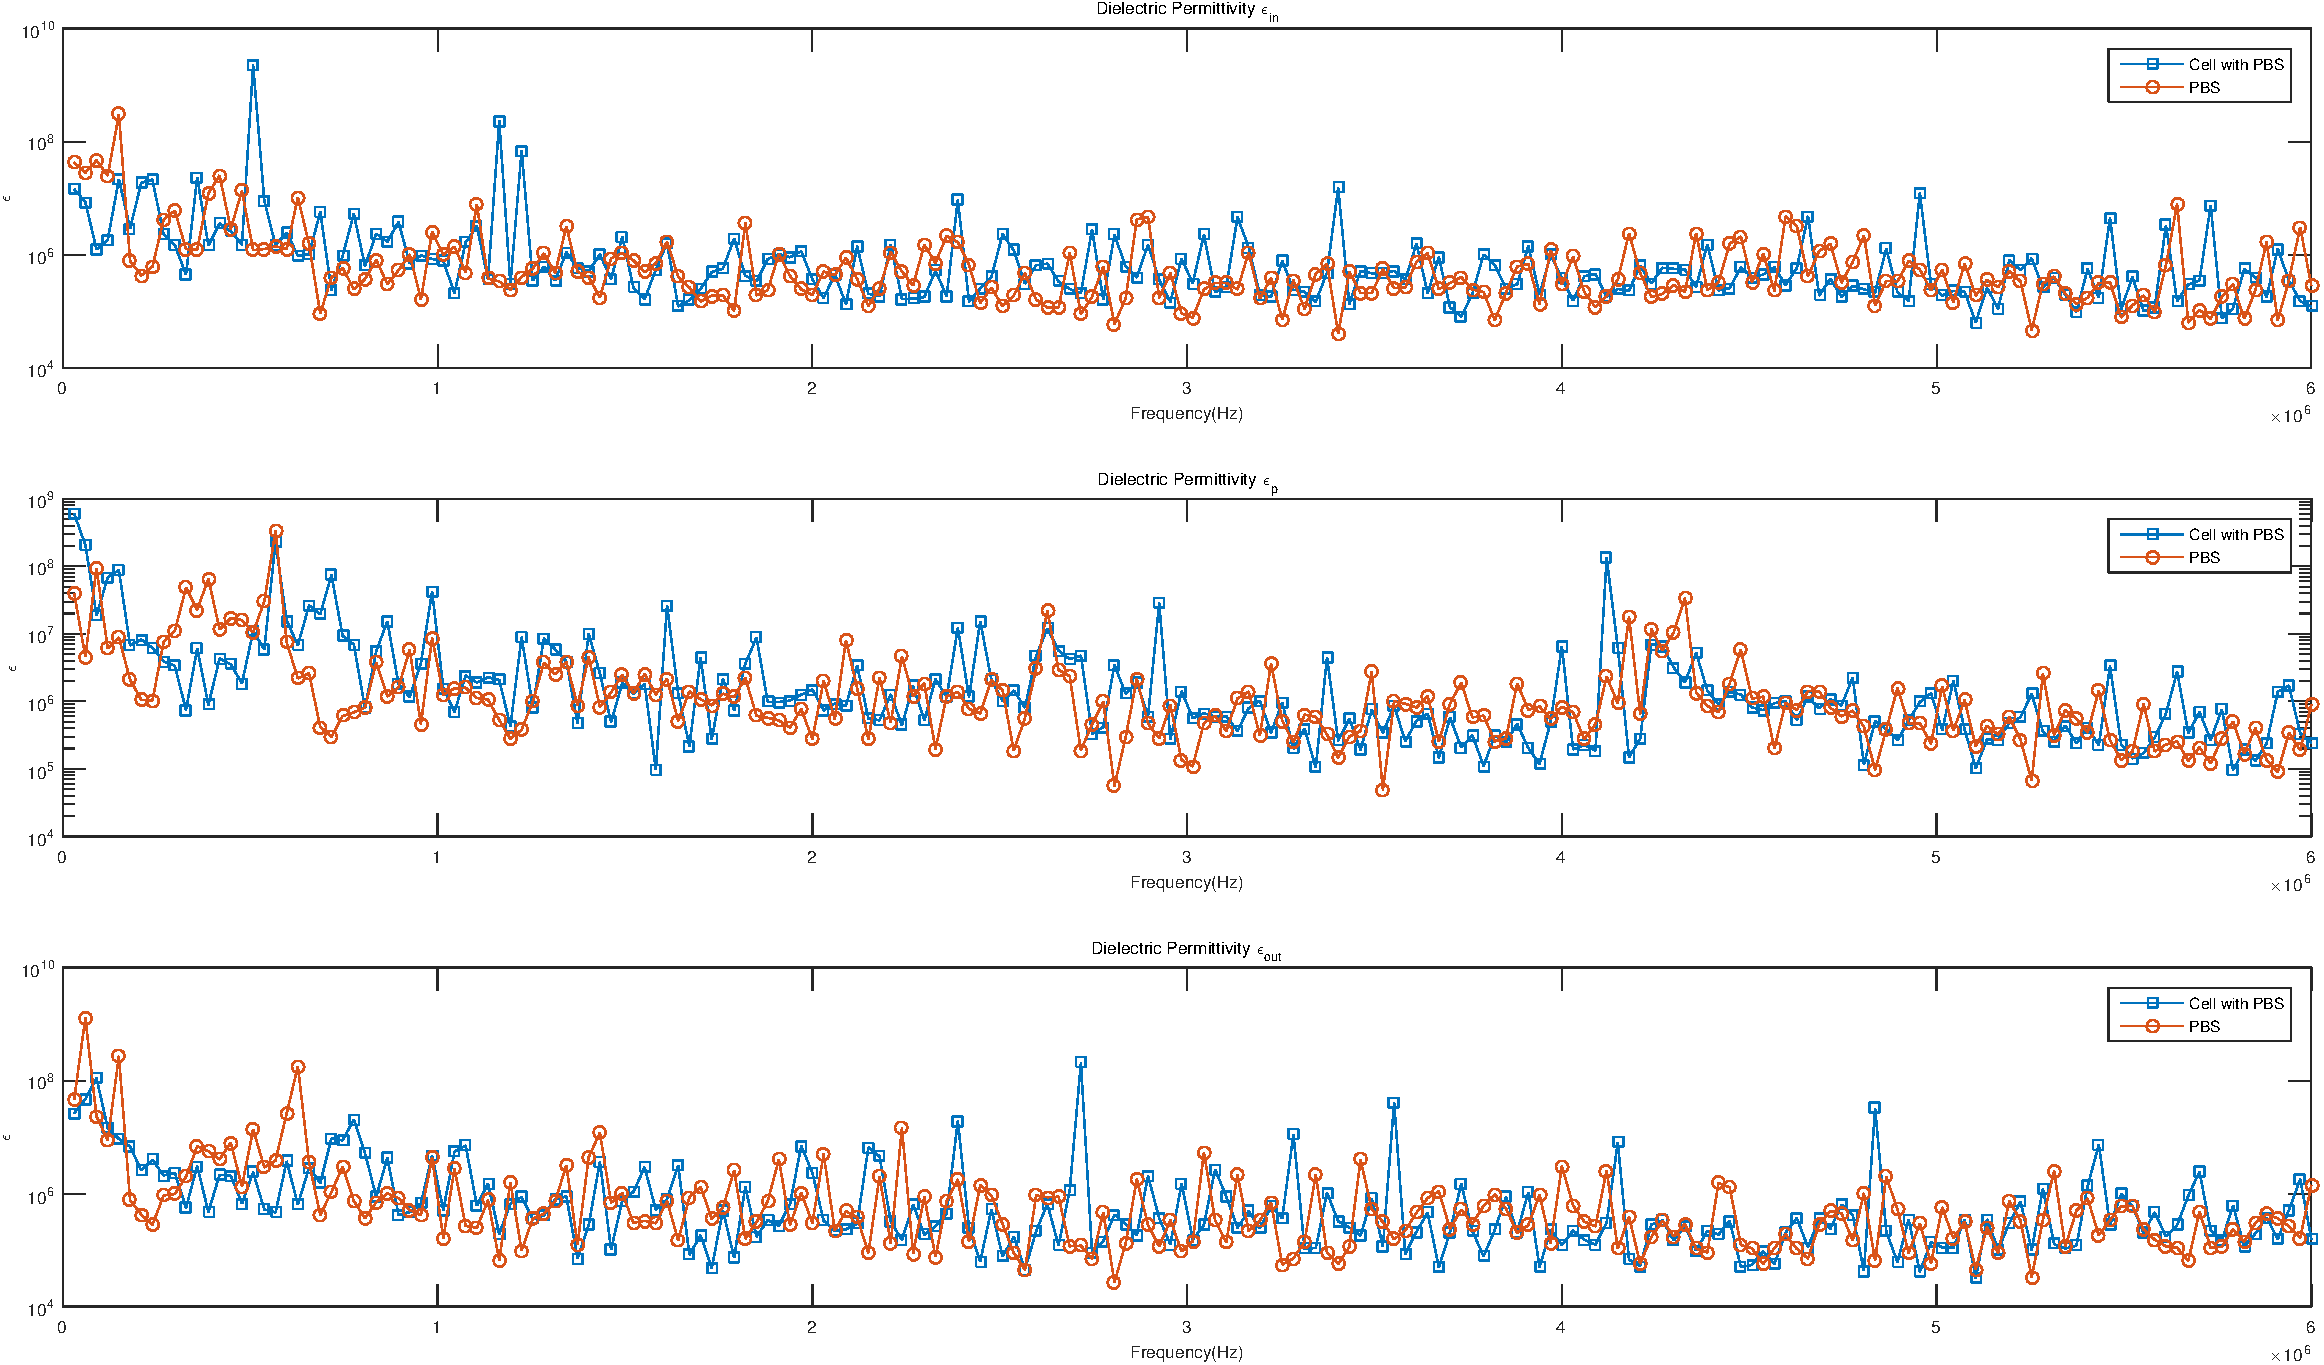
\includepdf[width = \textwidth]{dielectric_Permittivity.pdf}
\end{figure}

\end{document}
